%! Author = ben
%! Date = 18.02.2024

% Preamble

\documentclass[arbeitsmappe.tex]{subfiles}

% Document
\begin{document}

    \begin{gblock}{hinreichende Bedingung für Extrema mit 2. Ableitung}
        Die Funktion $f$ ist auf einem Intervall $I$ definiert und sowohl die Funktion als auch ihre erste Ableitung $f'$ sind differenzierbar. \\
        Wenn $f'(x) = 0$ und $f''(x) < 0$ gilt, so liegt ein Maximum vor. \\
        Wenn $f'(x) = 0$ und $f''(x) > 0$ gilt, so liegt ein Minimum vor. \\
    \end{gblock}

    \subsection{S. 21 Nr. 9}
    \begin{rblock}{Aufgabe}
        Gegeben sind die Funktionen f mit $f(x) = 0,25x^4 - x^3$ und g mit $g(x) = 0,2x^5 - 0,75x^4$. \\

        \paragraph{b)} Untersuchen Sie mithilfe der 2. Ableitung und mithilfe des Vorzeichenwechselkriteriums, ob die Graphen Hoch- und Tiefpunkte besitzen und skizzieren Sie den Verlauf der Graphen.
    \end{rblock}

    \begin{align*}
        f(x) &= 0.25x^4 - x^3 \\
        f'(x) &= x^3 - 3x^2 \\
        f''(x) &= 3x^2 - 6x
    \end{align*}

    notwendige Bedingung für EST: $f'(x) = 0$ \\
    \begin{align*}
        x^3 - 3x^2 &= 0 \\
        \Leftrightarrow x^3 - 3x^2 &= 0 \\
        \Leftrightarrow x^3 \times (x-3) &= 0 \\
        \Rightarrow x_1 &= 0 \\
        \Rightarrow x_2 &= 3
    \end{align*}

    hinreichende Bedingung für EST: $f'(x) = 0\ \land\ f''(x)\ne 0$ \\
    $\left.
    x_1:
    \begin{array}{ll}
        f''(0) = 3 \times 0^2 - 6 \times 0 \\
        f''(0) = 0                         \\
    \end{array}
    \right\} \Rightarrow \text{$f''(x) = 0$} \Rightarrow \text{Keine Extremstelle} \\
    $
    $\left.
    x_2:
    \begin{array}{ll}
        f''(3) = 3 \times 3^2 - 6 \times 3 \\
        f''(3) = 27-18                     \\
        f''(0) = 9                         \\
    \end{array}
    \right\} \Rightarrow \text{$f''(x) > 0$} \Rightarrow \text{Tiefpunkt} \\
    $
    \\
    hinreichende Bedingung für EST: $f'(x) = 0\ \land VZW$
    \\
    $\left.
    x_1:
    \begin{array}{ll}
        f'(-1) = (-1)^3 - 3\times (-1)^2 \\
        \Leftrightarrow f'(-1) = -1-3    \\
        \Leftrightarrow f'(-1) = -4      \\
        \\
        f'(1) = 1^3 - 3\times 1^2 \\
        \Leftrightarrow f'(1) = -2 \\
    \end{array}
    \right\} \Rightarrow \text{Kein Vorzeichenwechsel} \Rightarrow \text{Sattelpunkt} \\
    $
    \\[1cm]
    $\left.
    x_2:
    \begin{array}{ll}
        f'(2) = 2^3 - 3\times 2^2                \\
        \Leftrightarrow f'(2) = 8 - 12           \\
        \Leftrightarrow f'(2) = -4               \\
        \\
        f'(4) = 4^3 - 3\times 4^2 \\
        \Leftrightarrow f'(4) = 64 - 3 \times 16 \\
        \Leftrightarrow f'(4) = 64 - 48 \\
        \Leftrightarrow f'(4) = 16 \\
    \end{array}
    \right\} \Rightarrow \text{Vorzeichenwechsel von - zu +} \Rightarrow \text{Tiefpunkt} \\
    $
    \\
    \begin{align*}
        g(x) &= 0.2x^5 - 0.75x^4 \\
        g'(x) &= x^4 - 3x^3 \\
        g''(x) &= 4x^3 - 9x^2
    \end{align*}

    notwendige Bedingung für EST: $g'(x) = 0$ \\
    \begin{align*}
        x^4 - 3x^3 &= 0 \\
        \Leftrightarrow x^3 \times (x-3) &= 0 \\
        \Rightarrow x_1 &= 0 \\
        \Rightarrow x_2 &= 3
    \end{align*}

    hinreichende Bedingung für EST: $g'(x) = 0\ \land\ g''(x)\ne 0$ \\

    $\left.
    x_1:
    \begin{array}{ll}
        g''(0) = 4 \times 0^3 - 9 \times 0^2 \\
        g''(0) = 0                           \\
    \end{array}
    \right\} \Rightarrow \text{$g''(x) = 0$} \Rightarrow \text{Keine Extremstelle} \\
    $
    \\
    $\left.
    x_2:
    \begin{array}{ll}
        g''(3) = 4 \times 3^3 - 9 \times 3^2 \\
        g''(3) = 108-81                      \\
        g''(3) = 27                          \\
    \end{array}
    \right\} \Rightarrow \text{$g''(x) > 0$} \Rightarrow \text{Tiefpunkt} \\
    $
    \\
    hinreichende Bedingung für EST: $g'(x) = 0\ \land VZW$
    \\[1cm]
    $\left.
    x_1:
    \begin{array}{ll}
        g'(-1) = (-1)^4 - 3\times (-1)^3 \\
        \Leftrightarrow g'(-1) = 1+3     \\
        \Leftrightarrow g'(-1) = 4       \\
        \\
        g'(1) = 1^4 - 3\times 1^3 \\
        \Leftrightarrow g'(1) = -2 \\
    \end{array}
    \right\} \Rightarrow \text{Vorzeichenwechsel von + zu -} \Rightarrow \text{Hochpunkt} \\
    $
    \\[1cm]
    $\left.
    x_2:
    \begin{array}{ll}
        g'(2) = 2^4 - 3\times 2^3                 \\
        \Leftrightarrow g'(2) = 16 - 24           \\
        \Leftrightarrow g'(2) = -8                \\
        \\
        g'(4) = 4^4 - 3\times 4^3 \\
        \Leftrightarrow g'(4) = 256 - 3 \times 64 \\
        \Leftrightarrow g'(4) = 256 - 192 \\
        \Leftrightarrow g'(4) = 64 \\
    \end{array}
    \right\} \Rightarrow \text{Vorzeichenwechsel von - zu +} \Rightarrow \text{Tiefpunkt} \\
    $
    \newpage

    \subsection{S. 20 Nr. 4}

    \begin{rblock}{Aufgabe}
        Gegeben ist der Graph der Ableitungsfunktion $f'$.
        Welche der folgenden Aussagen sind richtig bzw. falsch? Begründen Sie.

        \paragraph{a)} f hat im abgebildeten Bereich zwei Extremstellen.

        \paragraph{b)} Die zweite Ableitung von f hat zwei Nullstellen.

        \paragraph{c)} Es gilt $f''(0) > 0$.

        \paragraph{d)} Der Graph von f hat an der Stelle $x = 0$ einen Hochpunkt.
    \end{rblock}

    \paragraph{a) } Ja, einen Tiefpunkt und einen Hochpunkt.

    \paragraph{b) } Ja, da es zwei Extremstellen und einen Sattelpunkt gibt.

    \paragraph{c) } Ja, da der Graph an einer Stelle immer langsamer steigt.

    \paragraph{d) } Nein, da der Graph an dieser Stelle einen Tiefpunkt hat.
    Im Intervall: Ränder sind globale Hoch- und Tiefpunkte.
    \newpage

    \subsection{S. 15 Nr. 15}
    \begin{rblock}{Aufgabe}
        Bläst man einen kugelförmigen Luftballon mit konstantem Luftstrom auf, so wächst der Radius des Ballons zu Beginn schneller als am Ende.
        Die Funktion $r(V)$ gibt ungefähr die Abhängigkeit des Radius $r$ vom Volumen $V$ an: $r(V) = \sqrt[3]{\frac{3V}{4\pi}}$

        \paragraph{a)} Zeichnen Sie den Graphen von $r$ und $r'$ mithilfe des GTR.

        \paragraph{b)} Bestimmen Sie die mittlere Änderungsrate für $r$ im Intervall $[0.5;1]$ und $[1;1.5]$.
        Interpretieren Sie das Ergebnis.

        \paragraph{c)} Skizzieren Sie mithilfe des GTR die Tangente an der Stelle $V_0 = 1$ und lesen Sie daraus die momentane Änderungsrate an dieser Stelle ab.
    \end{rblock}

    \paragraph{a) } \mbox{} \\
    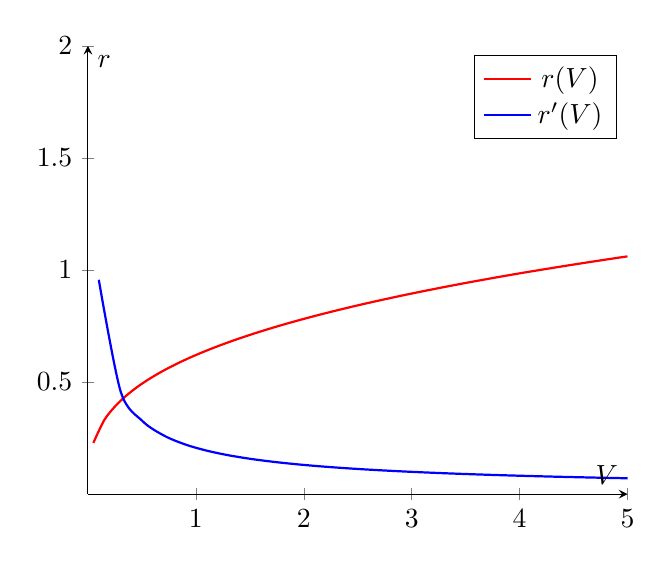
\begin{tikzpicture}
        \begin{axis}[
            axis lines = center,
            xlabel = $V$,
            ylabel = $r$,
            xmin=0,
            xmax=5,
            ymax=2,
            ymin=0
        ]
            \addplot [
                domain=-5:5,
                color=red,
                samples=100,
                smooth,
                thick,
            ]
            {((3*x)/(4*3.1415))^(0.3333)};
            \addlegendentry{$r(V)$}
            \addplot [
                domain=-10:10,
                samples=100,
                color=blue,
                smooth,
                thick,
            ]
            {(0.206783)/(x^0.6666)};
            \addlegendentry{$r'(V)$}
        \end{axis}
    \end{tikzpicture}

    \paragraph{b) } \mbox{} \\
    $
    \left.
    [0.5;1]
    \begin{array}{ll}
        \frac{r(1)-r(0.5)}{1-0.5} \\
        \xrightarrow{CAS} 0.18
    \end{array}
    \right\} \Rightarrow \text{Mittlere Änderungsrate} = 0.18 \\
    $
    Im Verlauf des Graphens wird die Steigung immer kleiner.

    \paragraph{c) } \mbox{} \\
    Die momentane Änderungsrate an der Stelle $V_0 = 1$ beträgt $\approx 0.21$

\end{document}
